\documentclass[journal]{IEEEtran}
\usepackage{amsmath,amssymb}
\usepackage{booktabs}
\usepackage{graphicx}
\usepackage{cite}
\usepackage{url}
\usepackage{siunitx}
\usepackage{tikz}
\usepackage{pgfplots}
\usetikzlibrary{arrows.meta,positioning}
\pgfplotsset{compat=1.18}

\title{Physics-Aware Configuration Selection for Phase-Coded FMCW Integrated Sensing and Communication in High-Mobility Vehicular Links}
\author{Anonymous Author(s)%
\thanks{Paper 1 is developed as a standalone PHY-level study from the repository's source-grounded waveform/profile evidence. Simulation results are explicitly separated from external measurements and from the later finite-sample reliability study.}}

% Standalone Paper 1 figures; values are derived from artifacts/stage7/pilot_validation.json.
\newcommand{\figPaperOneArchitecture}{%
\begin{figure*}[t]
\centering
\resizebox{\textwidth}{!}{%
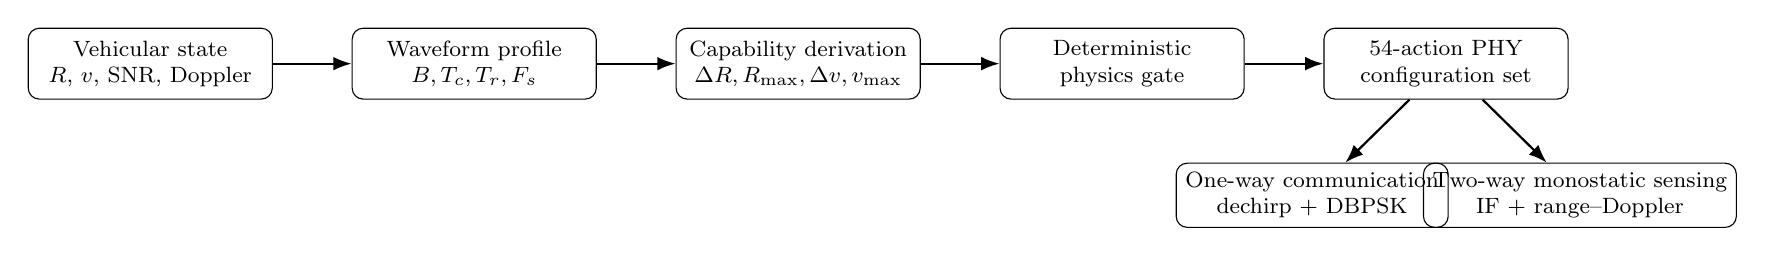
\begin{tikzpicture}[font=\footnotesize,node distance=8mm and 10mm,
box/.style={draw,rounded corners,align=center,minimum height=9mm,minimum width=31mm},
small/.style={draw,rounded corners,align=center,minimum height=8mm,minimum width=29mm},
arr/.style={-Latex,thick}]
\node[box] (state) {Vehicular state\\$R$, $v$, SNR, Doppler};
\node[box,right=of state] (profile) {Waveform profile\\$B,T_c,T_r,F_s$};
\node[box,right=of profile] (cap) {Capability derivation\\$\Delta R,R_{\max},\Delta v,v_{\max}$};
\node[box,right=of cap] (gate) {Deterministic\\physics gate};
\node[box,right=of gate] (action) {54-action PHY\\configuration set};
\node[small,below=of action,xshift=-17mm] (comm) {One-way communication\\dechirp + DBPSK};
\node[small,below=of action,xshift=17mm] (sens) {Two-way monostatic sensing\\IF + range--Doppler};
\draw[arr](state)--(profile);
\draw[arr](profile)--(cap);
\draw[arr](cap)--(gate);
\draw[arr](gate)--(action);
\draw[arr](action)--(comm);
\draw[arr](action)--(sens);
\end{tikzpicture}%
}%
\caption{Paper 1 architecture. Profile-level physical capability is derived before configuration selection. The communication path is one-way, while the sensing echo is two-way monostatic and processed at dechirped IF.}
\label{fig:p1architecture}
\end{figure*}%
}

\newcommand{\figPaper1Capability}{%
\begin{figure}[t]
\centering
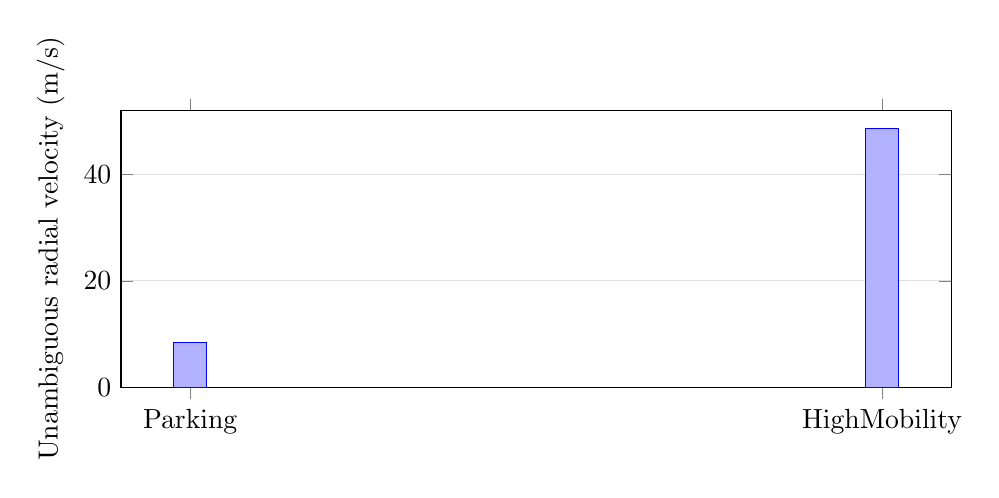
\begin{tikzpicture}
\begin{axis}[
width=\columnwidth,height=5.1cm,
ybar,bar width=12pt,ymin=0,ymax=52,
ylabel={Unambiguous radial velocity (m/s)},
symbolic x coords={Parking,HighMobility},xtick=data,
ymajorgrids=true,grid style={black!12}]
\addplot coordinates {(Parking,8.4055)(HighMobility,48.6676)};
\end{axis}
\end{tikzpicture}
\caption{Derived monostatic unambiguous radial-velocity support. The high-mobility capability profile extends the support by a factor of approximately 5.79 relative to the parking profile.}
\label{fig:p1capability}
\end{figure}%
}

\newcommand{\figPaper1Pilot}{%
\begin{figure*}[t]
\centering
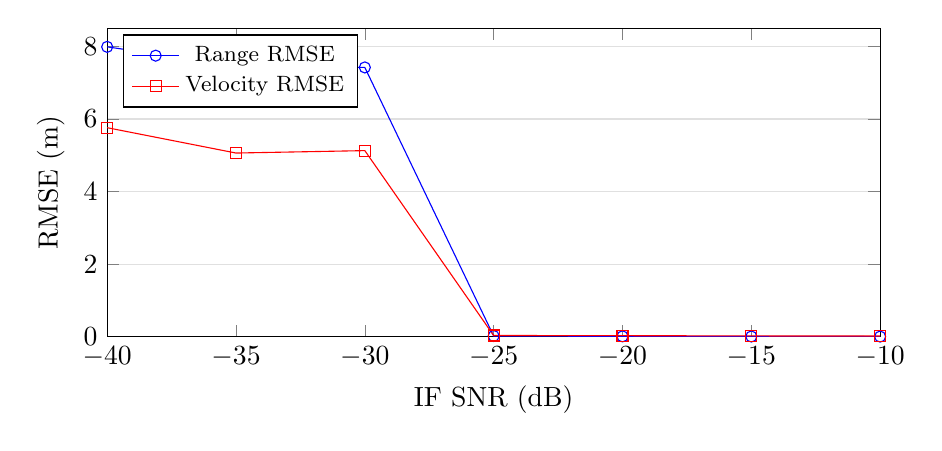
\begin{tikzpicture}
\begin{axis}[
width=0.94\textwidth,height=5.5cm,
xlabel={IF SNR (dB)},ylabel={RMSE (m)},
xmin=-40,xmax=-10,ymin=0,ymax=8.5,
legend style={font=\footnotesize,at={(0.02,0.98)},anchor=north west},
ymajorgrids=true,grid style={black!12}]
\addplot+[mark=o] coordinates {(-40,7.98657)(-35,7.46960)(-30,7.41971)(-25,0.02142)(-20,0.01151)(-15,0.00785)(-10,0.00560)};
\addplot+[mark=square] coordinates {(-40,5.75981)(-35,5.06158)(-30,5.12805)(-25,0.03511)(-20,0.03011)(-15,0.02290)(-10,0.02071)};
\legend{Range RMSE,Velocity RMSE}
\end{axis}
\end{tikzpicture}
\caption{Parking-profile pilot sensing evidence at $(R,v)=(10\,\mathrm{m},3\,\mathrm{m/s})$, 50 trials per SNR point. The sharp improvement around $-25$ dB is simulation evidence from the repository, not a hardware measurement.}
\label{fig:p1pilot}
\end{figure*}%
}


\begin{document}
\maketitle

\begin{abstract}
Integrated sensing and communication (ISAC) systems that reuse frequency-modulated continuous-wave (FMCW) signals for sensing and data transmission face a configuration constraint that is distinct from stochastic link quality: a candidate waveform may be attractive under nominal QoS metrics yet physically unable to represent the requested range or radial velocity. This paper studies that problem for a 77-GHz phase-coded FMCW (PC-FMCW) vehicular physical layer. We construct an interpretable 54-action space and formulate standard FMCW range and unambiguous-velocity limits as a state-dependent hard admissibility layer applied before QoS/resource ranking. A controlled gated-versus-ungated ablation keeps the action set, nominal QoS screen, and ranking identical and removes only this physical filter. On a declared boundary-aware range--velocity stress grid, 132 of 238 states are supportable by at least one action. Among these supportable states, the capability-blind selector chooses a physically unsupported action in 114 cases (86.36\%) despite the existence of a valid alternative, whereas physics-gated selection returns a physically valid action in all 132 states. Source-grounded profile analysis gives approximately 0.175-m range resolution and 8.41-m/s monostatic unambiguous radial velocity for the parking profile, while a composite high-mobility capability profile extends velocity support to approximately 48.67 m/s. Pilot simulations validate the declared sensing and DBPSK reference paths. The contribution is not a new FMCW capability equation, but an explicit physical-admissibility stage for finite-action PC-FMCW selection and controlled evidence of the recoverable selection failure caused by omitting it. The study is simulation/model based and does not claim hardware validation, field prevalence, or a commercial implementation of the composite high-mobility profile.
\end{abstract}

\begin{IEEEkeywords}
Integrated sensing and communication, phase-coded FMCW, automotive radar, vehicular communications, physical feasibility, range--Doppler sensing, adaptive PHY, 77 GHz.
\end{IEEEkeywords}

\section{Introduction}
Integrated sensing and communication (ISAC) aims to share waveform, spectrum, hardware, and signal-processing resources between wireless communication and environmental sensing \cite{liu2022isac,wang2022isac}. Vehicular operation is demanding because communication and sensing are exposed to rapid state variation, Doppler, interference, synchronization errors, and tight latency constraints \cite{wang2024isac,vehicular2022isac,ma2026vehicularisac}.

Phase-coded FMCW is attractive because an FMCW carrier preserves the delay--Doppler structure used by automotive radar while phase modulation provides a communication degree of freedom. Experimental and analytical PC-FMCW studies have established the waveform family and investigated receiver structures, smoothing, coherent MIMO operation, code-dependent sensing, performance, and interference mitigation \cite{kumbul2021experimental,kumbul2022receiver,kumbul2022smoothed,kumbul2022codes,kumbul2023mimo,kumbul2023performance,kumbul2024interference}. We do not introduce phase coding, a new modulation format, or a new range--Doppler estimator.

The key observation is architectural. Bandwidth determines range resolution, IF sampling and chirp slope constrain positive-IF range support, and repetition interval determines monostatic unambiguous radial velocity. These relations are standard; however, if finite candidate configurations are ranked without first enforcing their state-dependent support, a decision layer can select a waveform that cannot represent the requested state. Such deterministic support failure should not be delegated to a later stochastic reliability calculation.

This paper therefore: (i) defines a physically consistent joint communication/sensing model; (ii) derives profile-level capability boundaries; (iii) constructs an interpretable 54-action PC-FMCW space; and (iv) isolates the role of physical admissibility through a controlled gated-versus-ungated selector ablation.

The contributions are:
\begin{itemize}
\item a PC-FMCW signal model that distinguishes one-way communication from two-way monostatic sensing and dechirped-IF sampling;
\item an analytical capability layer that converts standard FMCW timing, bandwidth, and IF-sampling relations into a state-dependent admissible action set;
\item a finite 54-action PHY configuration space with directly interpretable control dimensions;
\item a controlled ablation in which only the physical filter is removed: among 132 supportable stress-grid states, the ungated selector chooses an unsupported action in 114 cases (86.36\%) despite a valid alternative, while the gated selector is physically valid in all 132;
\item source-grounded profile and pilot-simulation evidence with explicit separation between simulation and hardware measurement.
\end{itemize}

\section{Related Work}
The broader ISAC literature establishes dual-function waveform design and coupled sensing/communication resource trade-offs \cite{liu2022isac,wang2022isac,wang2024isac}. Vehicular ISAC adds rapid channel and target dynamics, making waveform timing, Doppler, synchronization, implementation constraints, and robustness particularly important \cite{vehicular2022isac,ma2026vehicularisac}.

PC-FMCW provides the closest waveform-specific background. Kumbul et al. experimentally investigated PC-FMCW sensing and communications and subsequently studied receiver structures, smoothed waveforms, coherent MIMO, sensing codes, performance, and interference mitigation \cite{kumbul2021experimental,kumbul2022receiver,kumbul2022smoothed,kumbul2022codes,kumbul2023mimo,kumbul2023performance,kumbul2024interference}. These works establish important waveform properties, including Doppler and unambiguous-velocity behavior, but address waveform/receiver design rather than the controlled finite-action admissibility ablation studied here.

Adaptive waveform and ISAC resource optimization are also established research areas; therefore neither adaptation itself nor physical FMCW limits are claimed as new. Recent radar-centric FMCW ISAC work, for example, dynamically reconfigures chirp duration, bandwidth, and phase coding to trade communication throughput against sensing performance \cite{temiz2026adaptive}. Our question is narrower: before a finite PC-FMCW action is ranked for QoS or resource cost, is that action physically capable of representing the requested range--velocity state? We encode that requirement as a hard first-stage admissibility set and remove only that set in a controlled counterfactual. Robust resource allocation and robust ISAC beamforming address uncertainty in channel state, target location, or optimization variables \cite{wu2021robustv2x,lyu2024dualrobust}; those methods are complementary to deterministic representability checks.

\section{System and Signal Model}
For chirp index $m$ and fast time $t$, the idealized transmitted signal is
\begin{equation}
s_m(t)=\sqrt{P_m}\exp\left(j[\pi\mu t^2+\phi_m(t)]\right),
\end{equation}
where $\mu=B/T_c$, $B$ is swept bandwidth, $T_c$ is active chirp duration, $P_m$ is transmit power, and $\phi_m(t)$ is the phase-coded communication waveform.

For monostatic sensing,
\begin{equation}
\tau_r=\frac{2R}{c},\qquad f_{D,r}=\frac{2vf_c}{c},\qquad f_b=\mu\tau_r+f_{D,r}.
\end{equation}
The receiver processes the dechirped beat/IF signal rather than directly sampling the 77-GHz carrier. The complex IF matrix is processed across fast and slow time with windowed FFTs; Doppler is estimated and removed from the beat-frequency estimate before range recovery under the simulator convention.

The remote communication path is one-way,
\begin{equation}
\tau_c=\frac{R}{c},\qquad f_{D,c}=\frac{vf_c}{c}.
\end{equation}
The reference modem uses multi-chip DBPSK after FMCW dechirping. Under AWGN, the noncoherent reference is
\begin{equation}
P_b=\frac{1}{2}\exp(-E_b/N_0).
\end{equation}

\section{Physical Capability Layer}
For each profile,
\begin{align}
\Delta R &= \frac{c}{2B}, & R_{\max}^{(+\mathrm{IF})} &= \frac{cF_s}{4\mu},\\
v_{\max} &= \frac{\lambda}{4T_r}, & \Delta v &= \frac{\lambda}{2N_cT_r}.
\end{align}
These are standard FMCW capability relations; the methodological step in this work is to make their state-dependent satisfaction a prerequisite for action ranking.

The source-grounded parking profile uses 77 GHz, $B=\SI{858}{MHz}$, $T_c=\SI{25.6}{\micro s}$, $T_r=\SI{115.8}{\micro s}$, $F_s=\SI{10}{MSPS}$, 256 samples/chirp, and 64 chirps/frame \cite{tiParking}. It gives approximately $\Delta R=\SI{0.175}{m}$, $R_{\max}^{(+\mathrm{IF})}=\SI{22.36}{m}$, $\Delta v=\SI{0.263}{m/s}$, and $v_{\max}=\SI{8.41}{m/s}$.

The composite high-mobility capability profile uses 77 GHz, $B=\SI{1}{GHz}$, $T_c=T_r=\SI{20}{\micro s}$, $F_s=\SI{37.5}{MSPS}$, 750 samples/chirp, and 128 chirps/frame. Its derived values are approximately $\Delta R=\SI{0.150}{m}$, $R_{\max}^{(+\mathrm{IF})}=\SI{56.21}{m}$, $\Delta v=\SI{0.760}{m/s}$, and $v_{\max}=\SI{48.67}{m/s}$. It is a capability reference, not a claimed commercial preset.

\begin{table}[t]
\centering
\caption{Source-grounded and derived profile capabilities.}
\label{tab:profiles}
\begin{tabular}{lcc}\toprule
Quantity & Parking & High mobility\\\midrule
Carrier & 77 GHz & 77 GHz\\
Bandwidth & 858 MHz & 1 GHz\\
Chirp/repetition & 25.6/115.8 $\mu$s & 20/20 $\mu$s\\
IF sampling & 10 MSPS & 37.5 MSPS\\
Range resolution & 0.175 m & 0.150 m\\
Positive-IF range & 22.36 m & 56.21 m\\
Velocity resolution & 0.263 m/s & 0.760 m/s\\
Unambiguous velocity & 8.41 m/s & 48.67 m/s\\\bottomrule
\end{tabular}
\end{table}

\section{Physics-Gated Finite Action Space}
The adaptive PHY action is
\begin{equation}
a=(p,N_{\rm chip},b,N_{\rm rep}),
\end{equation}
with two profiles, $N_{\rm chip}\in\{16,32,64\}$, power backoff $b\in\{0,3,6\}$ dB, and repetition $N_{\rm rep}\in\{1,2,4\}$, giving $|\mathcal A|=54$.

For estimated state $\hat S=(\hat R,\hat v,\ldots)$, the gate retains
\begin{equation}
\mathcal{A}_{\mathrm{phys}}(\hat S)=\{a\in\mathcal{A}:\hat R\le R_{\max}^{(+\mathrm{IF})}(a),\ |\hat v|\le v_{\max}(a)\}.
\end{equation}
If this set is empty, the state is physically infeasible for the declared action set. This is distinct from policy abstention or a low stochastic reliability estimate.

\section{Pilot Validation}
The repository pilot is simulation evidence, not measurement. For the parking target $(R,v)=(\SI{10}{m},\SI{3}{m/s})$ over 50 trials/SNR, range/velocity RMSE at $-25$ dB IF SNR are $\SI{0.0214}{m}$ and $\SI{0.0351}{m/s}$, compared with $\SI{7.42}{m}$ and $\SI{5.13}{m/s}$ at $-30$ dB. For the high-mobility capability profile at $R=\SI{20.28}{m}$ and $v=\SI{19.856}{m/s}$, the $-30$ dB range and velocity RMSE are approximately $\SI{0.0106}{m}$ and $\SI{0.0946}{m/s}$. The communication reference uses 32 chips/chirp and 300,000 bits per $E_b/N_0$ point; simulated DBPSK BER is 0.18363 versus 0.18394 theory at 0 dB and 0.00092 versus 0.00091 at 8 dB. These results validate the declared simulation paths, not a fielded vehicular link.

\figPaperOneCapability
\figPaperOnePilot
\section{Deterministic Physics-Gate Ablation}
To isolate the value of physical feasibility filtering from the later robust-policy study, we compare two deterministic nominal selectors over the same 54-action space. Both use the same nominal communication/sensing QoS screen and the same normalized-resource ranking. The only difference is that the gated selector first applies the canonical range and unambiguous-velocity support test, whereas the ungated selector ranks all actions without that test. No Monte-Carlo uncertainty draws, Wilson bounds, or B4 reliability qualification are used in this Paper 1 ablation.

The operating grid is deliberately boundary-aware rather than probabilistically weighted. It contains 14 range values from 0 to 60 m and 17 signed radial-velocity values from $-60$ to $60$ m/s, including samples immediately around the parking and high-mobility support boundaries. Of the resulting 238 states, 132 are physically representable by at least one declared profile and 106 are outside the support of the complete action set.

% AUTO-GENERATED from Paper 1 physics-gate ablation evidence; do not hand-edit.
\begin{table}[t]
\centering
\caption{Paper-1 deterministic physics-gate ablation on the boundary-aware range--velocity grid.}
\label{tab:p1gateablation}
\begin{tabular}{lrrrr}
\toprule
Selector & Selected & Selection rate & Invalid & Invalid/selected\\
\midrule
Gated & 132 & 55.46\% & 0 & 0.00\%\\
Ungated & 238 & 100.00\% & 220 & 92.44\%\\
\bottomrule
\end{tabular}
\end{table}


The ungated selector returns an action in all 238 states, but 220 selections (92.44\%) violate the selected profile's deterministic range or velocity support. This percentage characterizes the deliberately boundary-stressing grid and must not be interpreted as a prevalence estimate for real driving. The gated selector selects in the 132 supportable states and makes zero physically invalid selections. In 114 states, the ungated selector chooses an invalid configuration even though another action in the same 54-action set is physically valid; the gate exposes that valid alternative before nominal QoS ranking. In the remaining unsupported states, gating correctly distinguishes physical infeasibility of the declared action set from policy abstention.

% AUTO-GENERATED from Paper 1 physics-gate ablation evidence; do not hand-edit.
\newcommand{\figPaperOneGateAblation}{%
\begin{figure*}[t]
\centering
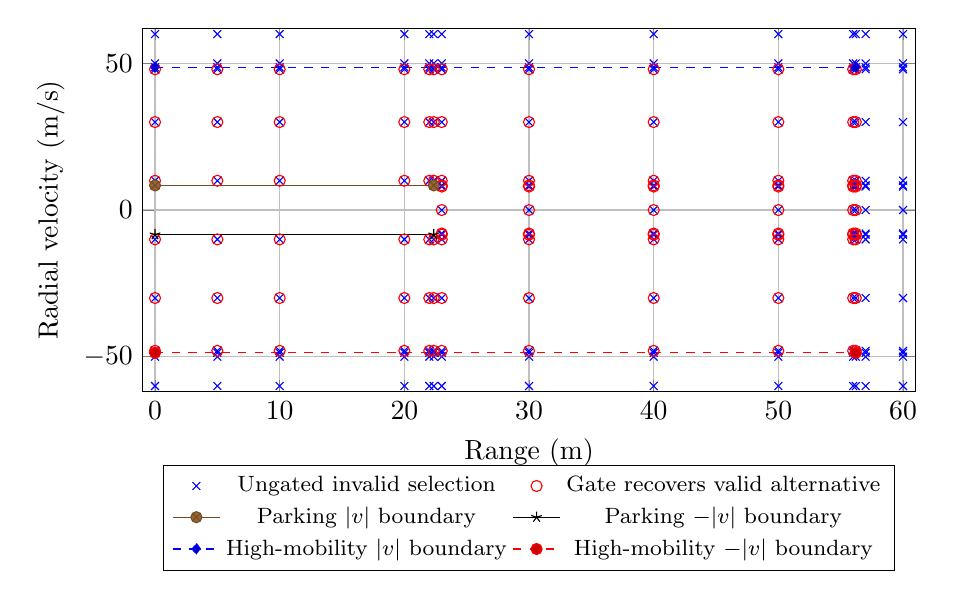
\begin{tikzpicture}
\begin{axis}[width=0.94\textwidth,height=6.2cm,xlabel={Range (m)},ylabel={Radial velocity (m/s)},xmin=-1,xmax=61,ymin=-62,ymax=62,grid=major,legend style={font=\footnotesize,at={(0.5,-0.20)},anchor=north,legend columns=2}]
\addplot+[only marks,mark=x] coordinates {(0,-60) (0,-50) (0,-48.67) (0,-48) (0,-30) (0,-10) (0,10) (0,30) (0,48) (0,48.67) (0,50) (0,60) (5,-60) (5,-50) (5,-48.67) (5,-48) (5,-30) (5,-10) (5,10) (5,30) (5,48) (5,48.67) (5,50) (5,60) (10,-60) (10,-50) (10,-48.67) (10,-48) (10,-30) (10,-10) (10,10) (10,30) (10,48) (10,48.67) (10,50) (10,60) (20,-60) (20,-50) (20,-48.67) (20,-48) (20,-30) (20,-10) (20,10) (20,30) (20,48) (20,48.67) (20,50) (20,60) (22,-60) (22,-50) (22,-48.67) (22,-48) (22,-30) (22,-10) (22,10) (22,30) (22,48) (22,48.67) (22,50) (22,60) (22.36,-60) (22.36,-50) (22.36,-48.67) (22.36,-48) (22.36,-30) (22.36,-10) (22.36,10) (22.36,30) (22.36,48) (22.36,48.67) (22.36,50) (22.36,60) (23,-60) (23,-50) (23,-48.67) (23,-48) (23,-30) (23,-10) (23,-8.41) (23,-8) (23,0) (23,8) (23,8.41) (23,10) (23,30) (23,48) (23,48.67) (23,50) (23,60) (30,-60) (30,-50) (30,-48.67) (30,-48) (30,-30) (30,-10) (30,-8.41) (30,-8) (30,0) (30,8) (30,8.41) (30,10) (30,30) (30,48) (30,48.67) (30,50) (30,60) (40,-60) (40,-50) (40,-48.67) (40,-48) (40,-30) (40,-10) (40,-8.41) (40,-8) (40,0) (40,8) (40,8.41) (40,10) (40,30) (40,48) (40,48.67) (40,50) (40,60) (50,-60) (50,-50) (50,-48.67) (50,-48) (50,-30) (50,-10) (50,-8.41) (50,-8) (50,0) (50,8) (50,8.41) (50,10) (50,30) (50,48) (50,48.67) (50,50) (50,60) (56,-60) (56,-50) (56,-48.67) (56,-48) (56,-30) (56,-10) (56,-8.41) (56,-8) (56,0) (56,8) (56,8.41) (56,10) (56,30) (56,48) (56,48.67) (56,50) (56,60) (56.21,-60) (56.21,-50) (56.21,-48.67) (56.21,-48) (56.21,-30) (56.21,-10) (56.21,-8.41) (56.21,-8) (56.21,0) (56.21,8) (56.21,8.41) (56.21,10) (56.21,30) (56.21,48) (56.21,48.67) (56.21,50) (56.21,60) (57,-60) (57,-50) (57,-48.67) (57,-48) (57,-30) (57,-10) (57,-8.41) (57,-8) (57,0) (57,8) (57,8.41) (57,10) (57,30) (57,48) (57,48.67) (57,50) (57,60) (60,-60) (60,-50) (60,-48.67) (60,-48) (60,-30) (60,-10) (60,-8.41) (60,-8) (60,0) (60,8) (60,8.41) (60,10) (60,30) (60,48) (60,48.67) (60,50) (60,60)};
\addplot+[only marks,mark=o] coordinates {(0,-48) (0,-30) (0,-10) (0,10) (0,30) (0,48) (5,-48) (5,-30) (5,-10) (5,10) (5,30) (5,48) (10,-48) (10,-30) (10,-10) (10,10) (10,30) (10,48) (20,-48) (20,-30) (20,-10) (20,10) (20,30) (20,48) (22,-48) (22,-30) (22,-10) (22,10) (22,30) (22,48) (22.36,-48) (22.36,-30) (22.36,-10) (22.36,10) (22.36,30) (22.36,48) (23,-48) (23,-30) (23,-10) (23,-8.41) (23,-8) (23,0) (23,8) (23,8.41) (23,10) (23,30) (23,48) (30,-48) (30,-30) (30,-10) (30,-8.41) (30,-8) (30,0) (30,8) (30,8.41) (30,10) (30,30) (30,48) (40,-48) (40,-30) (40,-10) (40,-8.41) (40,-8) (40,0) (40,8) (40,8.41) (40,10) (40,30) (40,48) (50,-48) (50,-30) (50,-10) (50,-8.41) (50,-8) (50,0) (50,8) (50,8.41) (50,10) (50,30) (50,48) (56,-48) (56,-30) (56,-10) (56,-8.41) (56,-8) (56,0) (56,8) (56,8.41) (56,10) (56,30) (56,48) (56.21,-48) (56.21,-30) (56.21,-10) (56.21,-8.41) (56.21,-8) (56.21,0) (56.21,8) (56.21,8.41) (56.21,10) (56.21,30) (56.21,48)};
\addplot+[domain=0:22.36,samples=2] {8.4055};
\addplot+[domain=0:22.36,samples=2] {-8.4055};
\addplot+[domain=0:56.21,samples=2,dashed] {48.6676};
\addplot+[domain=0:56.21,samples=2,dashed] {-48.6676};
\legend{Ungated invalid selection,Gate recovers valid alternative,Parking $|v|$ boundary,Parking $-|v|$ boundary,High-mobility $|v|$ boundary,High-mobility $-|v|$ boundary}
\end{axis}
\end{tikzpicture}
\caption{Boundary-aware Paper-1 ablation. Crosses mark states where the nominal ungated selector chooses a configuration outside its deterministic FMCW support; circles identify the subset for which physics gating instead exposes a valid alternative. Lines show the two profiles' unambiguous-velocity boundaries; range support is additionally enforced in the machine-readable evidence. This is deterministic analytical/simulation-model evidence, not a hardware measurement.}
\label{fig:p1gateablation}
\end{figure*}%
}

\figPaperOneGateAblation

The ablation therefore supports a narrow methodological claim: standard FMCW capability relations become operationally important when they are enforced as a hard first-stage constraint in finite-action configuration selection. It does not show that all ungated ISAC controllers fail, nor does it establish field reliability. Its purpose is to demonstrate a concrete selection failure mode that cannot be repaired by subsequent statistical averaging once an unsupported waveform has already been chosen.


\section{Discussion}
The profile calculations show why physical support must be separated from stochastic performance. The parking profile offers fine range and velocity resolution but only about 8.41 m/s unambiguous radial-velocity support; a state near 19.86 m/s cannot be made representable by increasing SNR or Monte-Carlo sample count. The high-mobility profile expands this support to approximately 48.67 m/s at greater sampling burden.

The ablation makes the architectural point stronger than profile calculations alone. Conditioning on the 132 states for which at least one declared action is physically valid, the capability-blind selector is valid in only 18 cases and invalid in 114 despite an available valid alternative. These 114 cases are recoverable configuration-selection errors, not globally impossible states. The gated selector returns a valid action in all 132 supportable states. Across the full 238-state boundary-stress grid, 220 ungated selections are invalid, but that secondary 92.44\% statistic includes 106 states outside the support of the complete action set and is therefore not a field-prevalence estimate.

The zero-invalid gated result is expected from the definition of the admissibility layer; the informative counterfactual is that removing only this layer while retaining the same action set, nominal QoS screen, and resource ranking creates 114 recoverable invalid decisions. The experiment does not claim that all other ISAC controllers are capability blind. It isolates the consequence of allowing ranking to operate on actions whose waveform cannot represent the state.

Accordingly, the novelty claim is not the FMCW equations themselves and not adaptive waveform selection in general. It is the explicit decision architecture that maps known capability relations into a state-dependent admissible action set before finite PC-FMCW ranking, together with a controlled ablation that quantifies the failure mode when this stage is omitted. Reliability under uncertain SNR, Doppler/synchronization, interference, or state estimation is a separate question and belongs to the subsequent reliability study.

\section{Limitations and Claim Boundaries}
This is a PHY-level model/simulation study. The boundary-aware grid is intentionally constructed to stress profile transitions and must not be interpreted as a distribution of real driving states. The parking parameters are grounded in published Texas Instruments reference-design documentation; the high-mobility profile is a composite capability reference and is not a commercial preset. Pilot results are not RF measurements. The paper does not claim trajectory prediction, planning, scheduling, beam management, standards compliance, embedded-ECU timing, universal superiority, or real-world reliability. The resource dimensions are interpretable control indices rather than measured energy.

\section{Conclusion}
This paper formulated deterministic FMCW range--velocity representability as a hard first-stage admissibility layer for finite-action 77-GHz PC-FMCW ISAC configuration selection. On the declared boundary-aware stress grid, 132 states admit at least one valid action; without the capability filter, 114 of these 132 supportable states (86.36\%) receive an unsupported selection despite a valid alternative, whereas gated selection returns physically valid actions in all 132. This controlled counterfactual, rather than the standard FMCW equations themselves, is the central evidence for preventing QoS/resource ranking from operating on physically unsupported actions. Source-grounded profile calculations and pilot simulations provide the supporting PHY context while preserving strict simulation/hardware boundaries. The resulting design principle is deliberately ordered: deterministic physical admissibility first, stochastic reliability qualification second.

\bibliographystyle{IEEEtran}
\bibliography{paper1_references}
\end{document}
